\documentclass[conference]{IEEEtran}
\IEEEoverridecommandlockouts{}

\usepackage{cite}
\usepackage{amsmath,amssymb,amsfonts}
\usepackage{algorithmic}
\usepackage{graphicx}
\usepackage{textcomp}
\usepackage{xcolor}
\usepackage{tabularx}
\usepackage{float}

\def\BibTeX{{\rm B\kern-.05em{\sc i\kern-.025em b}\kern-.08em
    T\kern-.1667em\lower.7ex\hbox{E}\kern-.125emX}}
\begin{document}

\title{Programación lineal ejecutada con el método de Gauss-Seidel\\}

\author{\IEEEauthorblockN{1\textsuperscript{st} Mauro Alonso Gonzalez Figueroa}
    \IEEEauthorblockA{\textit{Universiddad Tecnologica de Bolivar} \\
        \textit{UBT}\\
        Cartagena, Colombia \\
        maugonzalez@utb.edu.co}
    \and
    \IEEEauthorblockN{2\textsuperscript{nd} German De Armas Castaño}
    \IEEEauthorblockA{\textit{Universidad Tecnologica de Bolivar} \\
        \textit{UTB}\\
        Cartagena, Colombia \\
        gdearmas@utb.edu.co}
    \and
    \IEEEauthorblockN{3\textsuperscript{rd} Angel Vega Rodriguez}
    \IEEEauthorblockA{\textit{Universidad Tecnologica de Bolivar} \\
        \textit{UTB}\\
        Cartagena, Colombia \\
        anvega@utb.edu.co}
}

\maketitle

\bibliographystyle{IEEETran}

\begin{abstract}
    In the realm of numerical analysis, the Gauss-Seidel method stands as an
    iterative technique employed to resolve systems of linear equations. It
    represents a refined version of the Jacobi method, often exhibiting
    superior convergence properties. Within the scope of this paper, we delve
    into the application of the Gauss-Seidel method to address a system of
    linear equations arising from a financial planning conundrum. Our
    endeavor demonstrates the efficacy and efficiency of the Gauss-Seidel
    method in tackling this type of system.
\end{abstract}

\begin{IEEEkeywords}
    Gauss-Seidel method, linear equations, financial planning
\end{IEEEkeywords}

\nocite{*}

\section{Introduction}
En el ámbito de la gestión empresarial, la Investigación de Operaciones
\textit{(IO)} se erige como una herramienta fundamental para la optimización de
procesos y la toma de decisiones estratégicas. Esta disciplina, basada
en el método científico y el análisis matemático, permite a las
organizaciones abordar problemas complejos de manera sistemática y
eficiente, conduciéndolas hacia el logro de sus objetivos.

En esencia, la IO se caracteriza por la aplicación de un enfoque
interdisciplinario que integra conocimientos de diversas áreas, como
las matemáticas, la estadística, la ingeniería y la economía. Este
enfoque colaborativo permite a los equipos de trabajo abordar problemas
complejos desde múltiples perspectivas, generando soluciones innovadoras
y efectivas.

\section{Gauss-Seidel}

Dentro del amplio arsenal de técnicas empleadas en la IO, el método
Gauss-Seidel se destaca como un algoritmo iterativo de gran utilidad para
la resolución de sistemas de ecuaciones lineales. Este método, ampliamente
reconocido por su simplicidad y eficiencia, se basa en la actualización
progresiva de las variables del sistema en función de las aproximaciones
más recientes de las demás. A través de un proceso iterativo, las
estimaciones se van refinando hasta alcanzar un punto de convergencia, donde
las soluciones satisfacen los criterios establecidos.

En el contexto de la programación lineal, el método Gauss-Seidel cobra
especial relevancia como herramienta complementaria al método simplex. Si
bien el método simplex se considera el enfoque tradicional para resolver
este tipo de problemas, el método Gauss-Seidel ofrece una alternativa viable
para abordar problemas de gran escala o aquellos con características
específicas que dificultan la aplicación del simplex.

\section{Marco Teorico}

\subsection{Programación lineal}

La programación lineal es una técnica de modelización matemática desarrollada
a partir de la década de 1930. Desde entonces, se ha aplicado con
frecuencia en los procesos de toma de decisión de numerosos ámbitos
económicos y productivos. La técnica de programación lineal proporciona
soluciones las soluciones abiertas \textit{(no son formulas estrictas ni
    nada por el estilo)}, que más bien se determinan mediante algoritmos.

\begin{figure}[H]
    \begin{center}
        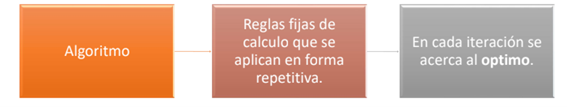
\includegraphics[width=\linewidth]{./Images/ProgramacionLineal.png}
        \caption{}
    \end{center}
\end{figure}

Algunos lineamientos generales para la implementación de la IO en la práctica.

\begin{enumerate}
    \item Definición del problemas
    \item Construcción del modelo
    \item Solución del modelo
    \item Validación del modelo
    \item implementación de la solución
\end{enumerate}

\subsection{Método o algebra simplex}

El Método Simplex es un método analítico de solución de problemas de 
programación lineal capaz de resolver modelos complejos. Aunque es un 
procedimiento algebraico, sus conceptos fundamentales son geométricos. 
El Simplex es un método iterativo que permite ir mejorando la solución en 
cada paso. El método consiste en caminar de vértice en vértice de manera que 
aumente o disminuya la función objetivo (según el criterio). Si existe el 
poliedro factible, el número de vértices que presenta es finito.

\begin{figure}[H]
    \begin{center}
        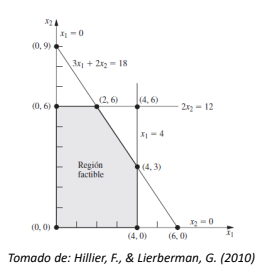
\includegraphics[width=.7\linewidth]{./Images/MetodoSimplex.png}
        \caption{}
    \end{center}
\end{figure}

\begin{figure}[H]
    \begin{center}
        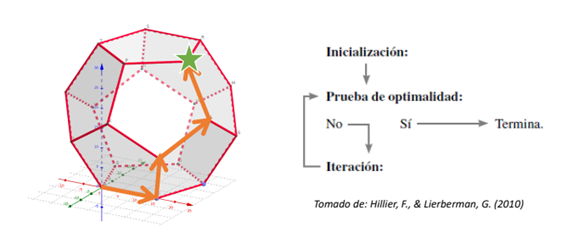
\includegraphics[width=\linewidth]{./Images/MetodoSimplex2.png}
        \caption{}
    \end{center}
\end{figure}

\subsection{Método de Gauss-Seidel}

Es un algoritmo utilizado para resolver sistemas de ecuaciones lineales. Es 
una variante del método de relajación y es especialmente útil cuando se 
trabaja con matrices grandes y densas.

En términos básicos, el método de Gauss-Seidel procede iterativamente, 
actualizando cada variable de un sistema de ecuaciones en función de las 
aproximaciones más recientes de las otras variables. En cada iteración, las 
nuevas estimaciones se utilizan para mejorar las aproximaciones de las 
variables restantes. Este proceso continúa hasta que las soluciones convergen 
a un valor aceptable.

El método de Gauss-Seidel puede ser más eficiente computacionalmente que 
otros métodos para resolver sistemas de ecuaciones lineales, especialmente 
cuando se trata de sistemas que son diagonales dominantes o simétricos 
positivos definidos. Sin embargo, su convergencia no está garantizada para 
todos los sistemas, y puede ser lento o incluso divergente en algunos casos. 
Por lo tanto, a veces se requieren ajustes o técnicas adicionales para 
garantizar la convergencia adecuada.

\subsection{Vector gradiente}

También conocido como vector gradiente (denotado $\nabla$f), es un 
campo vectorial que indica la dirección en la cual el campo f varía más 
rápidamente y su módulo representa el ritmo de variación de f en la dirección 
de dicho vector gradiente.

\begin{figure}[H]
    \begin{center}
        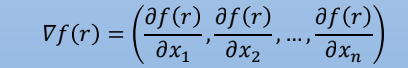
\includegraphics[width=\linewidth]{./Images/VectorGradiente.png}
        \caption{}
    \end{center}
\end{figure}

\subsection{Precio sombra}

El precio sombra puede representar una disposición a pagar por unidad 
adicional de recurso. Si el precio del recurso es menor al precio sombra 
entonces existirá un incentivo a ``comprar'' más debido a que esto tendrá un 
impacto neto positivo en la función objetivo.



\bibliography{./Bibliography/bibliography.bib}

\end{document}
